\documentclass[11pt]{article}  
\usepackage[margin=1in]{geometry}
\parindent=0in
\parskip=8pt
\usepackage{fancyhdr,amssymb,amsmath, graphicx, listings,float,subfig,enumerate,epstopdf,color,multirow,setspace,bm,textcomp}
\usepackage[usenames,dvipsnames]{xcolor}
\usepackage{hyperref}
\usepackage{graphicx}
\graphicspath{{./Images}}

\pagestyle{fancy}

\begin{document} 

\lhead{Assignment \#  7}
\chead{Robert Denim Horton}
\rhead{\today}

\begin{center}\begin{Large}
CS 4720 Networks, Crowds, and Markets

Homework \# 7

Student: (Robert Denim Horton)
\end{Large}
\end{center}

\section*{Answers to homework problems:}

\section*{Chapter 9}

% Question 1
\begin{enumerate}
	 \item In this question we will consider an auction in which there is one seller who wants to sell one unit of a good and a group of bidders who are each interested in purchasing the good. The seller will run a sealed-bid, second-price auction. Your firm will bid in the auction, but it does not know for sure how many other bidders will participate in the auction. There will be either two or three other bidders in addition to your firm. All bidders have independent, private values for the good. Your firm’s value for the good is c. What bid should your firm submit, and how does it depend on the number of other bidders who show up? Give a brief (1-3 sentence) explanation for your answer 
\end{enumerate}
% Question 1 Answers
\textcolor{gray}{
Answers:
\begin{enumerate}
	\item For the bidder of a particular firm, we denote the firm of intrest as $F$, their fixed self-set value for the good is denoted as $c$. We know from previous discussions in class that bidder $F$ should just bid what they think the item is worth.  While this does not guarantee that $F$ will win the auction, the probability of winning is independent of the other self-set values from other firms (either one or two more).  So, we can say that the value $c$ should be bided as there is no way of knowing if the other bidders will bid higher or lower, ultimately not changing what the best bid would be.  \\
\end{enumerate}
}

% Question 7
\begin{enumerate}
	\setcounter{enumi}{6}
	\item A seller announces that he will sell a case of rare wine using a sealed-bid, second-price auction. A group of individuals plan to bid on this case of wine. Each bidder is interested in the wine for his or her personal consumption; the bidders’ consumption values for the wine may differ, but they don’t plan to resell the wine. So we will view their values for the wine as independent, private values (as in Chapter 9). You are one of these bidders; in particular, you are bidder number i and your value for the wine is $V_i$.\\\\
How should you bid in each of the following situations? In each case, provide an explanation for your answer; a formal proof is not necessary.
	\begin{enumerate}
		\item  You know that a group of the bidders will collude on bids. This group will chose one bidder to submit a “real bid” of v and the others will all submit bids of 0. You are not a member of this collusive group and you cannot collude with any other bidder. \\\\
		\item You, and all of the other bidders, have just learned that this seller will collect bids, but won’t actually sell the wine according to the rules of a second-price auction. Instead, after collecting the bids the seller will tell all of the bidders that some other fictional bidder actually submitted the highest bid and so won the auction. This bidder,
of course, doesn’t exist so the seller will still have the wine after the auction is over. The seller plans to privately contact the highest actual bidder and tell him or her that the fictional high bidder defaulted (he didn’t buy the wine after all) and that this bidder can buy the wine for the price he or she bid in the auction. You cannot collude with any bidder. [You do not need to derive an optimal bidding strategy. It is enough to explain whether your bid would differ from your value and if so in what direction.]
	\end{enumerate}
\end{enumerate}
% Question 7 Answers
\textcolor{gray}{
Answers:
\begin{enumerate}
	\setcounter{enumi}{6}
	\item \quad\\
	\begin{enumerate}
		\item  Considering that a group of colluding bidders all submit a bid of 0, except for one of the colluding bidders that will submit a bid of a fixed value, $v$. While this tactic might seem to decrease your chances of winning the bid, the bid you set for what you think the item is valued at  is still independently set and will not change the odds regardless of what value the one collusive bidder that didn't bet 0, bids.   \\\\
		\item Now that we know that the actioner is cheating and the non-colluding bidders are not allowed to collude with any other biders, all the bidders are incentivised to underbid as although it is shaped as a first-price auction, opposed to what it advertisved as, a second-price auction. \\\\
	\end{enumerate}
\end{enumerate}
}

% Chapter 10
\section*{Chapter 10}

% Question 2
\begin{enumerate}
	\setcounter{enumi}{1}
	\item  Suppose we have a set of 3 sellers labelled a, b, and c, and a set of 3 buyers labelled x, y, and z. Each seller is offering a distinct house for sale, and the valuations of the buyers for the houses are as follows.
	\begin{center}
		% Uncomment to insert picture from Homeworkxx/Images
		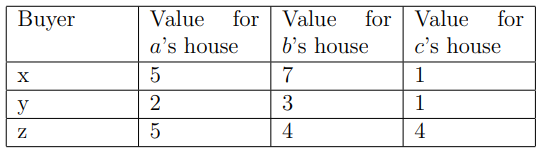
\includegraphics[scale=1.5]{Figure1.1}\\
		Figure 1.1
	\end{center}
Suppose that sellers a and b each charge 2, and seller c charges 1. Is this set of prices
market-clearing? Give a brief explanation.
\end{enumerate}
% Question 2 Answers
\textcolor{gray}{
Answers:
\begin{enumerate}
	\setcounter{enumi}{1}
	\item If there is a perfect matching, as defined in class, in a graph then we also can say that the current prices are \textit{market-clearing}.  By looking at Figure 1.2 we see a bipartite graph for the table provided in Figure 1.1.  
	\begin{center}
		% Uncomment to insert picture from Homeworkxx/Images
		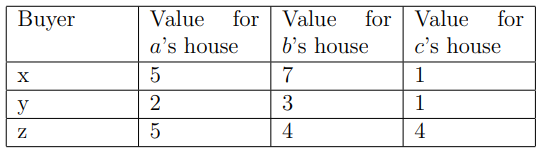
\includegraphics[scale=1.5]{Figure1.1}\\
		Figure 1.1
	\end{center}
	\begin{center}
		% Uncomment to insert picture from Homeworkxx/Images
		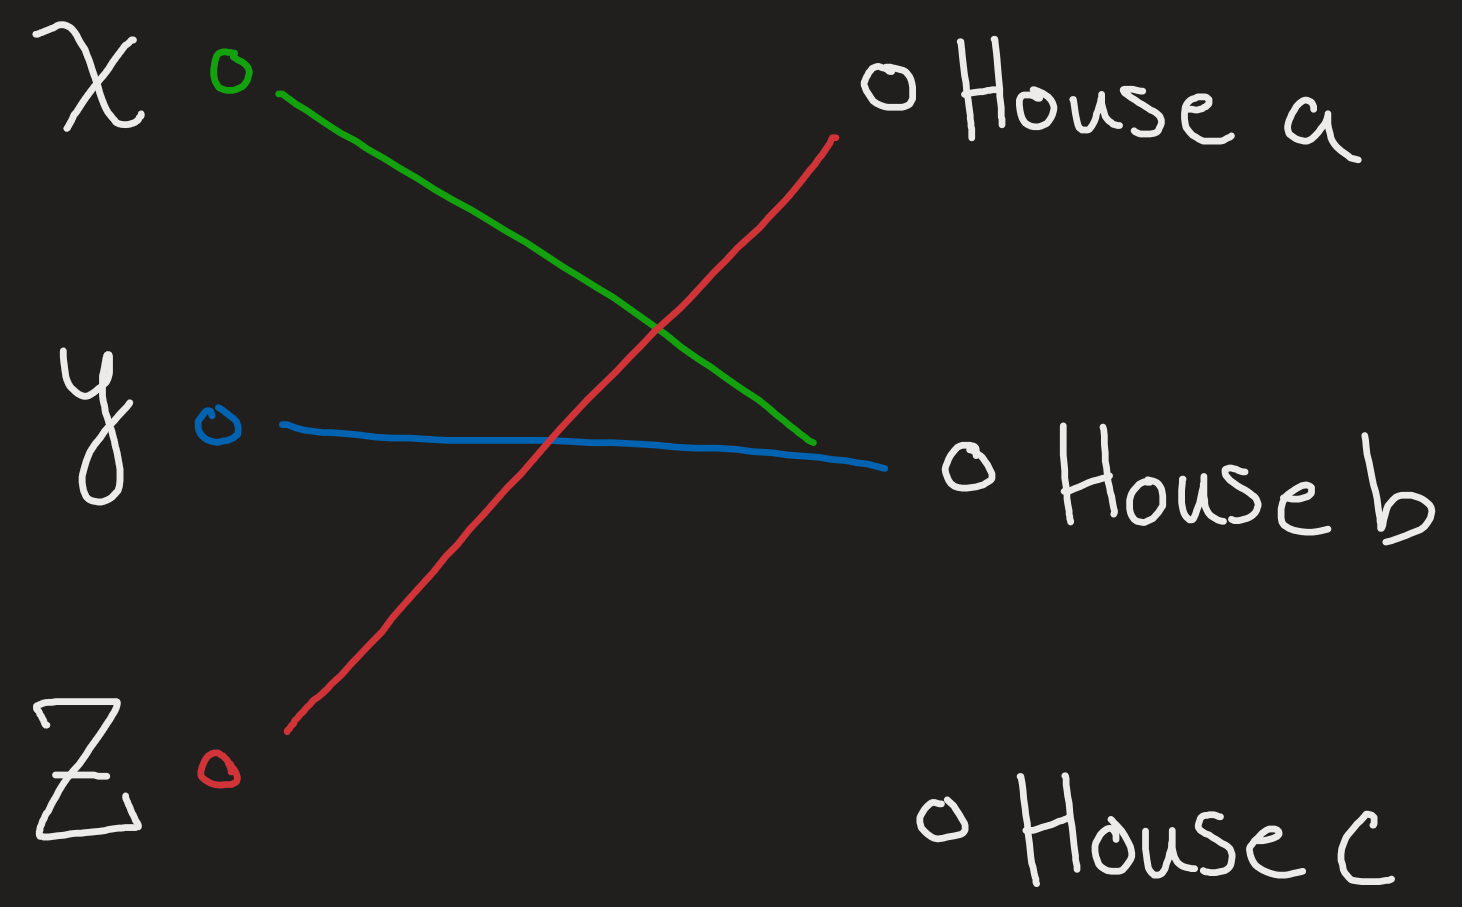
\includegraphics[scale=0.3]{Figure1.2}\\
		Figure 1.2
	\end{center}
  By observing the table and graph we see that buyers $x$ and $y$ share a mutual maximized desire for house $b$.  By considering the changes the the sellers values we see that the values drop to values displayed in Figure 1.3
	\begin{center}
		% Uncomment to insert picture from Homeworkxx/Images
		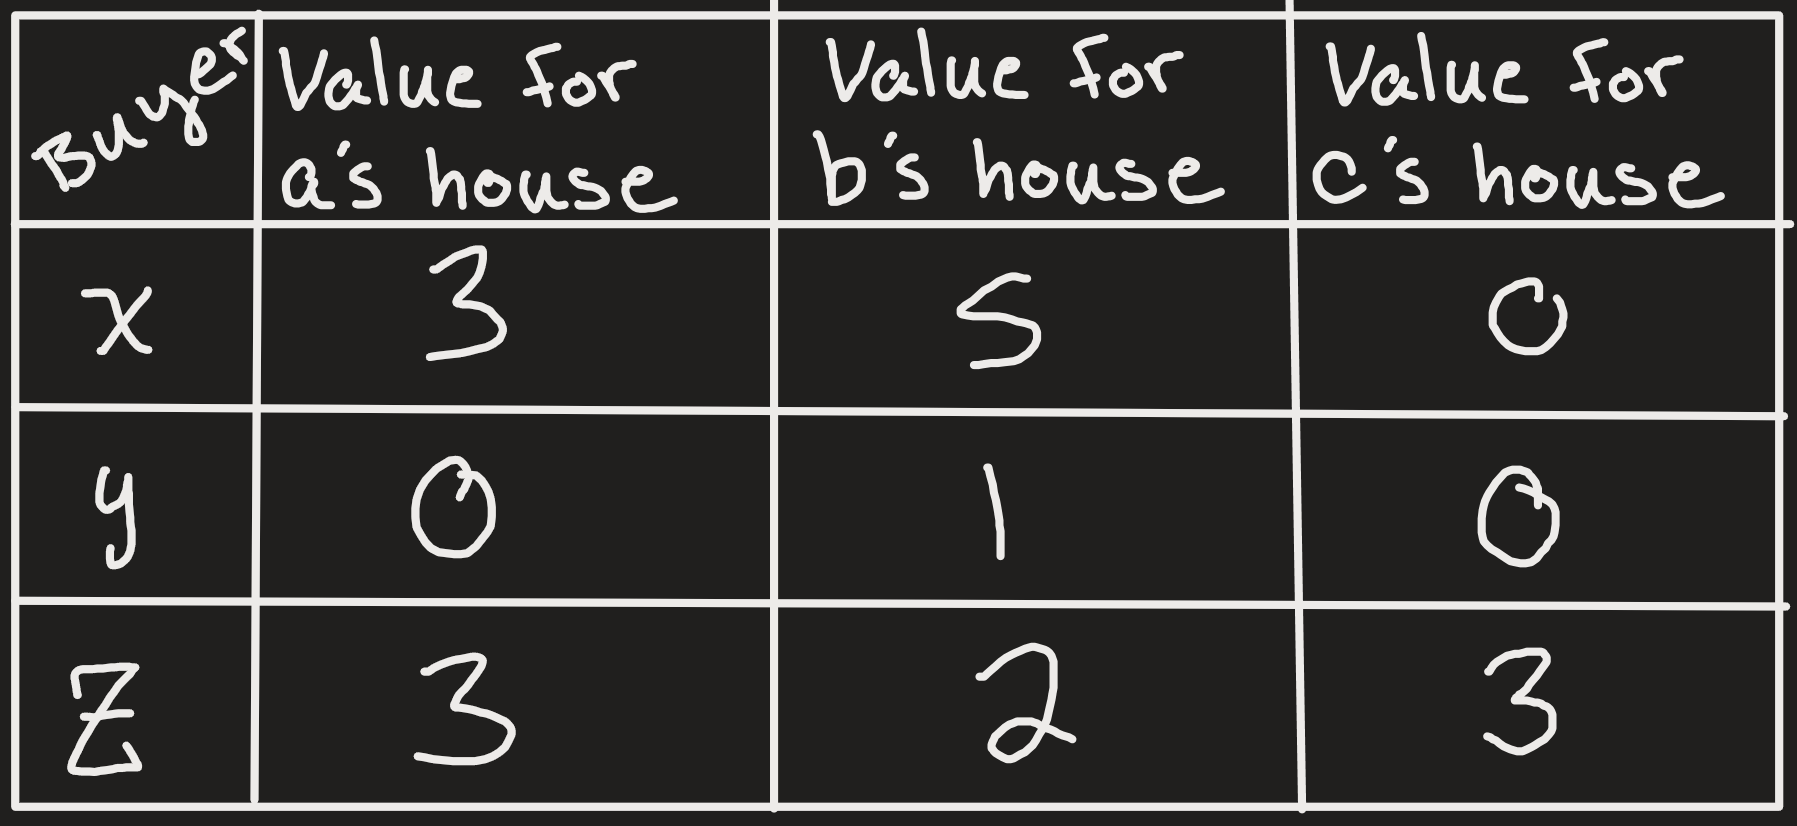
\includegraphics[scale=0.3]{Figure1.3}\\
		Figure 1.3
	\end{center}
\end{enumerate}
With this we see that there does not exist a perfect matching as buyers $y$ and $x$ share maximized desires for house $b$ and their fore no marketing-clearing set for the current prices either.
}
	
% Question 3
\begin{enumerate}
	\setcounter{enumi}{2}
	\item Suppose we have a set of 3 sellers labelled a, b, and c, and a set of 3 buyers labelled x, y, and z. Each seller is offering a distinct house for sale, and the valuations of the buyers for the houses are as follows.
	\begin{center}
		% Uncomment to insert picture from Homeworkxx/Images
		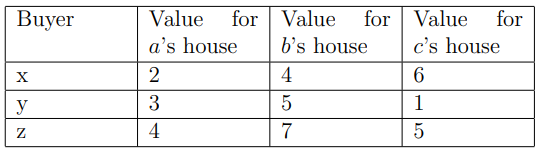
\includegraphics[scale=1.5]{Figure1.4}\\
		Figure 1.4
	\end{center}
Suppose that sellers a and c each charge 1, and seller b charges 3. Is this set of prices market-clearing? Give a brief explanation.
\end{enumerate}
% Question 3 Answers
\textcolor{gray}{
Answers:
\begin{enumerate}
	\setcounter{enumi}{2}
	\item By looking at the table in Figure 1.4 we see that the buyers $y$ and $z$ both want to have house $b$.  After performing the specified value changes for each buyer we that in figure 1.5 that the buyers $x$, $y$, and $z$ are a perfect matching.  So we can say that the current prices are a perfect market-clearing.
	\begin{center}
		% Uncomment to insert picture from Homeworkxx/Images
		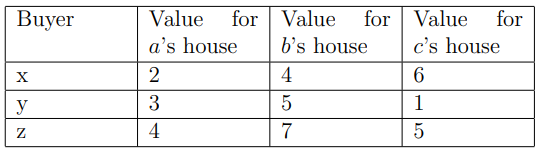
\includegraphics[scale=1.5]{Figure1.4}\\
		Figure 1.4
	\end{center} 
	\begin{center}
		% Uncomment to insert picture from Homeworkxx/Images
		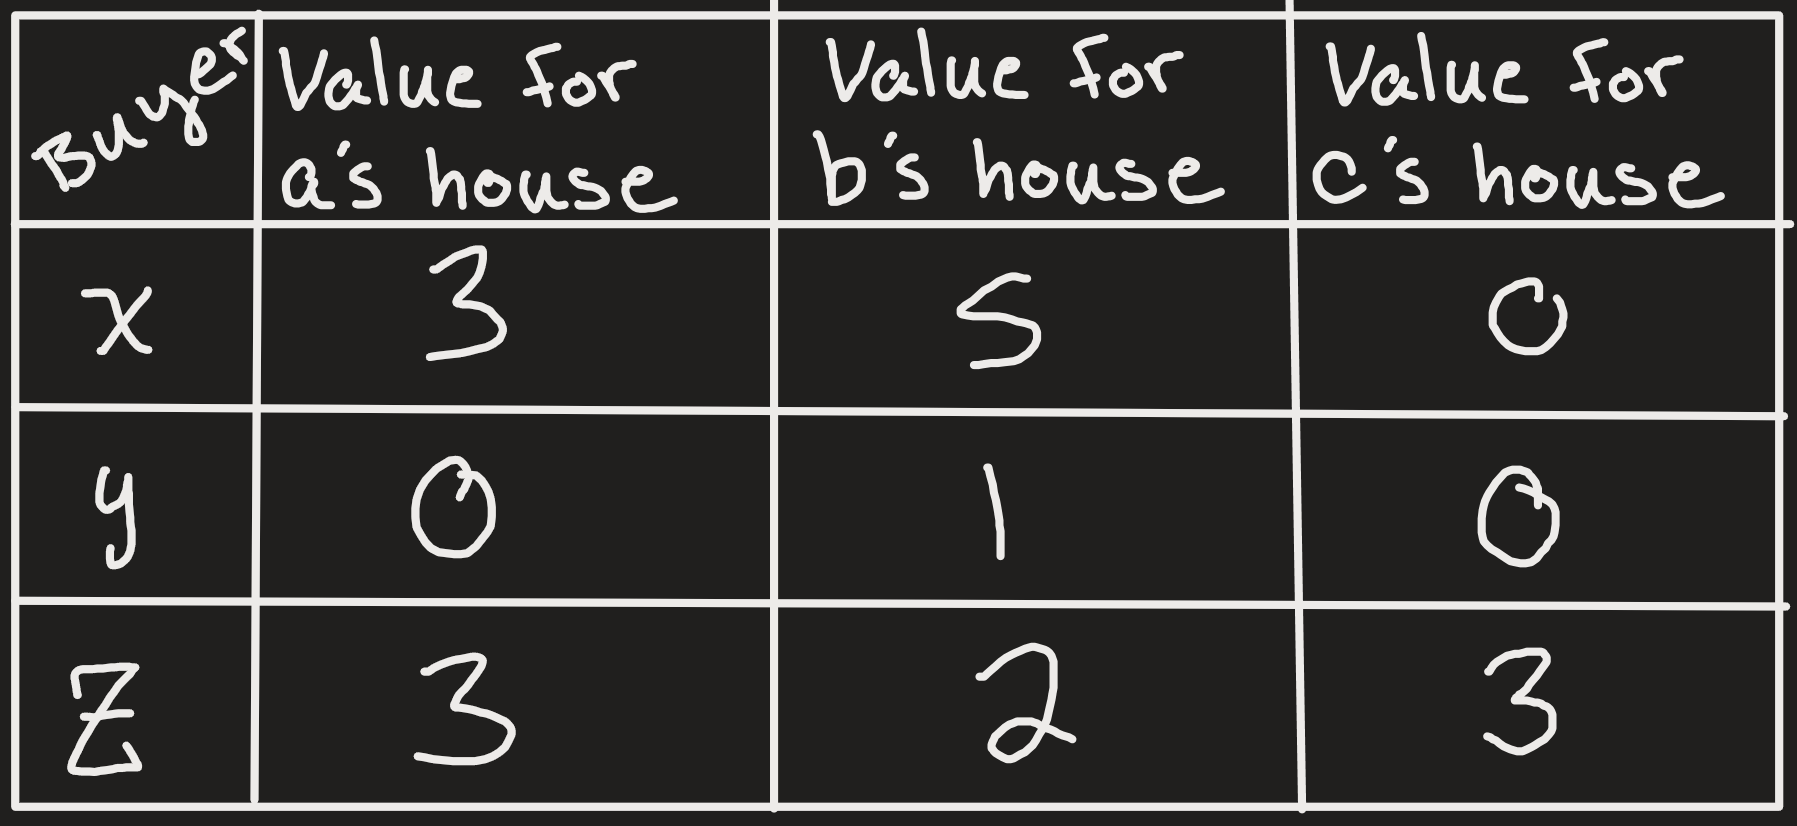
\includegraphics[scale=0.3]{Figure1.5}\\
		Figure 1.5d
	\end{center}
\end{enumerate}
}

	% Question 4
\begin{enumerate}
	\setcounter{enumi}{3}
	\item Suppose we have a set of 3 sellers labelled a, b, and c, and a set of 3 buyers labelled x, y, and z. Each seller is offering a distinct house for sale, and the valuations of the buyers for the houses are as follows.
	\begin{center}
		% Uncomment to insert picture from Homeworkxx/Images
		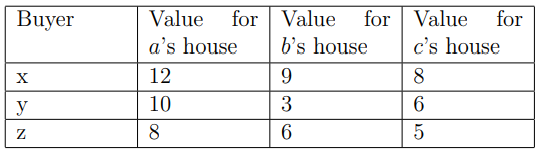
\includegraphics[scale=1.5]{Figure1.6}\\
		Figure 1.6
	\end{center}
Suppose that a charges a price of 3 for his house, b charges a price of 1 for his house, and c charges a price of 0. Is this set of prices market-clearing? If so, explain which buyer you would expect to get which house; if not, say which seller or sellers should raise their price(s) in the next round of the bipartite-graph auction procedure from Chapter 10.
\end{enumerate}
% Question 4 Answers
\textcolor{gray}{
Answers:
\begin{enumerate}
	\setcounter{enumi}{3}
	\item By building the graph suggested in the question, we get a table built with these values as shown in Figure 1.7.  We see by looking at this graph that it is not a perfect matching and therefore can not be market clearing.  Furthermore, the constricted set of sellers formed by set $S$ and $N(S)$ include $a$.  So we can say that $a$ should increase its price in the next round.
	\begin{center}
		% Uncomment to insert picture from Homeworkxx/Images
		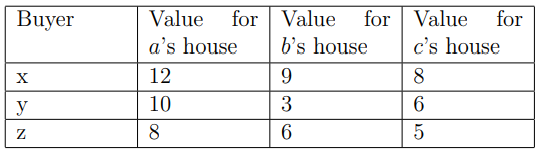
\includegraphics[scale=1.5]{Figure1.6}\\
		Figure 1.6
	\end{center}	\begin{center}
		% Uncomment to insert picture from Homeworkxx/Images
		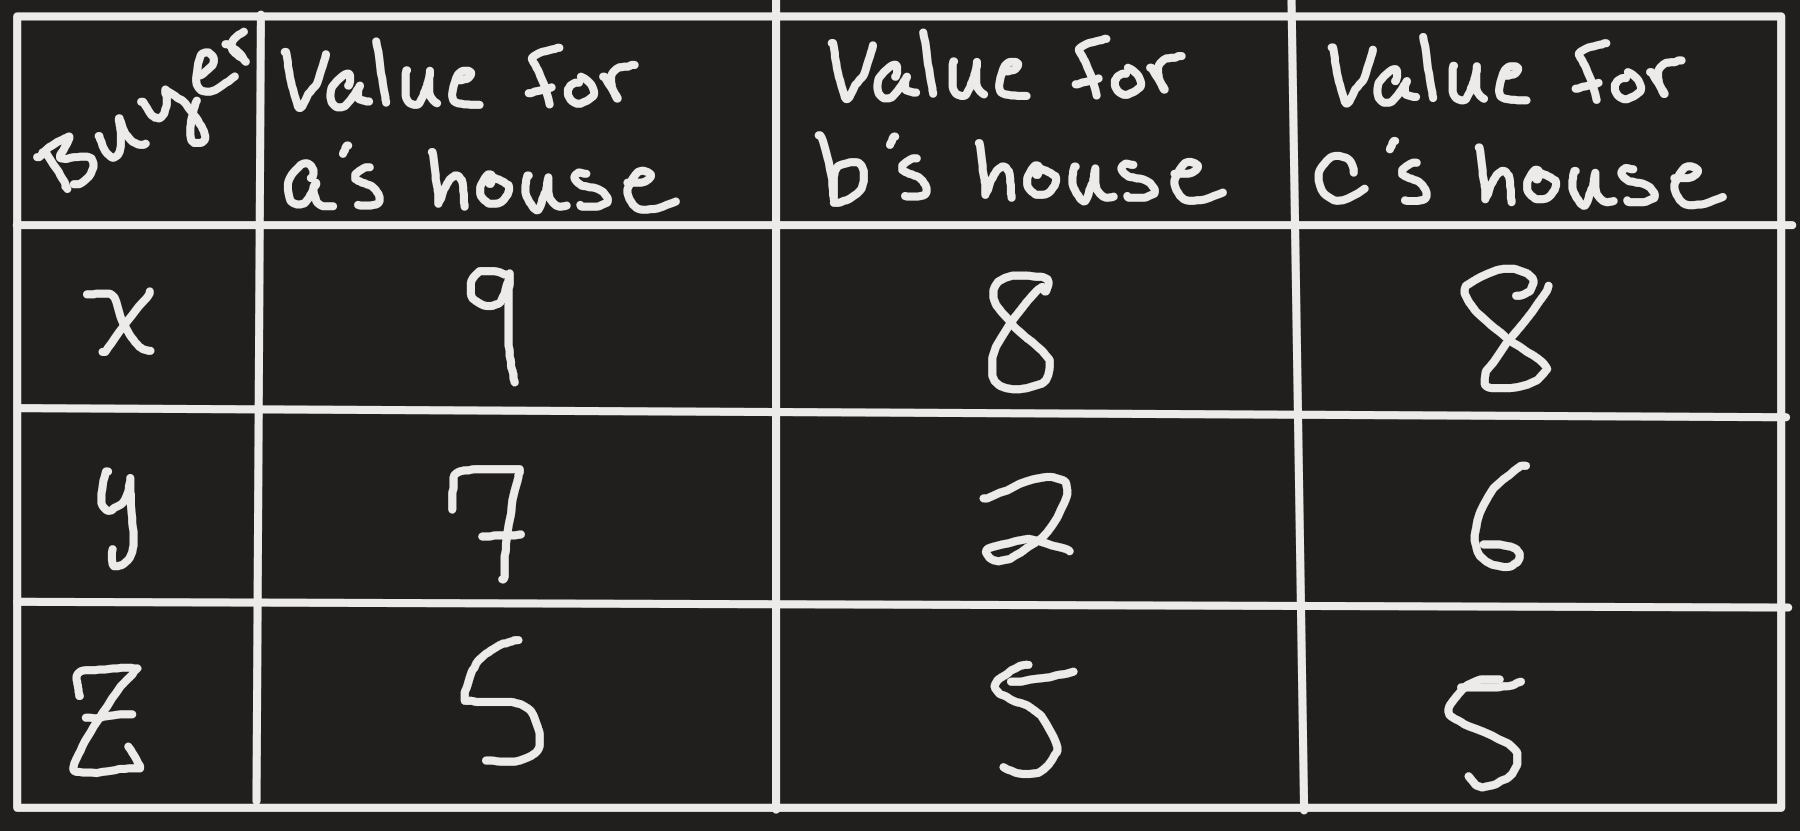
\includegraphics[scale=0.3]{Figure1.7}\\
		Figure 1.7
	\end{center}
\end{enumerate}
}
\end{document}
